

\documentclass[12pt]{report}
\usepackage[a4paper]{geometry}
\usepackage[myheadings]{fullpage}
\usepackage{fancyhdr}
\usepackage{lastpage}
\usepackage{graphicx, wrapfig, subcaption, setspace, booktabs}
\usepackage[T1]{fontenc}
\usepackage[font=small, labelfont=bf]{caption}
\usepackage{fourier}
\usepackage[protrusion=true, expansion=true]{microtype}
\usepackage[english]{babel}
\usepackage{sectsty}
\usepackage{url, lipsum}
\usepackage{tgbonum}
\usepackage{hyperref}
\usepackage{xcolor}

\newcommand{\HRule}[1]{\rule{\linewidth}{#1}}
\onehalfspacing
\setcounter{tocdepth}{5}
\setcounter{secnumdepth}{5}


\documentclass[a4paper,12pt]{article}
\usepackage[utf8]{inputenc}

% Default fixed font does not support bold face
\DeclareFixedFont{\ttb}{T1}{txtt}{bx}{n}{12} % for bold
\DeclareFixedFont{\ttm}{T1}{txtt}{m}{n}{12}  % for normal

% Custom colors
\usepackage{color}
\definecolor{deepblue}{rgb}{0,0,0.5}
\definecolor{deepred}{rgb}{0.6,0,0}
\definecolor{deepgreen}{rgb}{0,0.5,0}

\usepackage{listings}

% Python style for highlighting
\newcommand\pythonstyle{\lstset{
language=Python,
basicstyle=\ttm,
otherkeywords={self},             % Add keywords here
keywordstyle=\ttb\color{deepblue},
emph={MyClass,__init__},          % Custom highlighting
emphstyle=\ttb\color{deepred},    % Custom highlighting style
stringstyle=\color{deepgreen},
frame=tb,                         % Any extra options here
showstringspaces=false            % 
}}


% Python environment
\lstnewenvironment{python}[1][]
{
\pythonstyle
\lstset{#1}
}
{}

% Python for external files
\newcommand\pythonexternal[2][]{{
\pythonstyle
\lstinputlisting[#1]{#2}}}

% Python for inline
\newcommand\pythoninline[1]{{\pythonstyle\lstinline!#1!}}


%-------------------------------------------------------------------------------
% HEADER & FOOTER
%-------------------------------------------------------------------------------
\pagestyle{fancy}
\fancyhf{}
\setlength\headheight{15pt}
\fancyhead[L]{COSC560: MapReduce on Cloudlab}
\fancyhead[R]{Nguyen, Offutt}

%-------------------------------------------------------------------------------
% TITLE PAGE
%-------------------------------------------------------------------------------

\begin{document}
{\fontfamily{cmr}\selectfont
\title{ \normalsize \textsc{}
		\\ [2.0cm]
		\HRule{0.5pt} \\
		\LARGE \textbf{\uppercase{Programming Assignment 2: MapReduce on Cloudlab}
		\HRule{2pt} \\ [0.5cm]
		\normalsize{COSC560} \\
		\normalsize \today \vspace*{5\baselineskip}}
		}

\date{}

\author{
		Clara Nguyen \\ 
		Rachel Offutt \\
		University of Tennessee EECS }

\maketitle
\tableofcontents
\newpage

%-------------------------------------------------------------------------------
% Section title formatting
\sectionfont{\scshape}
%-------------------------------------------------------------------------------

%-------------------------------------------------------------------------------
% BODY
%-------------------------------------------------------------------------------

\section{Project Summary}
\indent {In this assignment,you will program the Map Reduce parallel data processing system on the Cloudlab cloud computing platform. This will allow you gain practical experience on Map Reduce programming and learn the performance implications of parallel data processing. The following basic goals must be fulfilled:
}
\indent \indent \begin{itemize}
    \item Cloudlab setup
    \item Create Cloudlab cluster on Hadoop
    \item Build the MapReduce code for the Reverse-indexer
    \item Run the MapReduce program on the Hadoop cluster
    \item Query the inverted index
\end{itemize}
%\newpage
%\section{Getting Started}
%\input{getstart.tex}


\section{Project Specific Requirements}
\subsection{Identifying and removing stop words}
One issue is that some words are so common that their presence in an inverted index is "noise," that is they can obfuscate the more interesting properties of a document. Such words are called “stop words.” For this part of the assignment, write a word count Map Reduce function to perform a word count over a corpus of text files and to identify stop words. It is up to you to choose a reasonable threshold (word count frequency) for stop words, but make sure you provide adequate justification and explanation of your choice. A parser will group words by attributes which are not relevant to their meaning (e.g.,"hello","Hello", and "HELLO" are all the same word), so it is up to you to  define "scrub" however you wish; some suggestions include case-insensitivity, etc. It is not required that you treat “run” and “ran” as the same word, but your parser should handle case insensitivity. Once you have written your code, then run your code and collect the word counts for submission with all your Mapper and Reducer files. 
\subsection{Building the Inverted Index}
For this portion of the assignment, you  will design a MapReduce-based algorithm to calculate the inverted index. To this end, you are to create a full inverted index, which maps words to their document ID + line number in the document. Note that your final inverted index should not contain the words identified in Step 1. The format of your MapReduce output (i.e.,the inverted index) must be simple enough to be machine-parseable; it is not impossible to imagine your index being one of many data structures used  in a search engine's indexing pipeline. Your submitted indexer should be  able to run successfully on one or multiple input txt files, where "successfully" means it should run to completion without errors or exceptions, and generate the correct word->DocID mapping. You are required to submit all relevant Mapper and Reducer Java files, in addition to any supporting code or utilities. 
\subsection{Query the Inverted Index}
Write a query program on top of your full inverted file index that accepts a user-specified query (one or more words) and returns not only the document IDs but also the locations in the form of line numbers. The query program can be local: it does not need to handle the task using Map-Reduce framework again. It is not required that your query program to return text snippets from the original text files.

\section{Project Design Choices}


    \subsection{Language Choice}
    We chose to implement this project in Python to gain more experience in this programming language and because of how well documented Python sockets are. 
    \subsection{Configuration}
    The application must be fine-tunable. As such, this webserver has a config JSON that is named config.json. This file is loaded at run-time and contains data on where essential directories are, as well as host and port values. This is what it may look like:
    \begin{verbatim}
    {
        "page_root": "./htdocs",
        "uploads": "./uploads",
        "host": "",
        "port": 28961
    } \end{verbatim}
    The following keys are required: \\
page\_root - Root directory of all webpages. \\
    uploads - Directory to store uploads.\\
    host - Host address (Leave blank for "localhost")\\
    port - Port number for server
    \subsection{Python Sockets}
    In this project, we are not allowed to use HTTP.sever, however, we were allowed and encouraged to use Python sockets. Since we previously decided that our programming language would be Python, the only way to complete this project would be with the use of Python sockets.
    \subsection{Threading}
        Modern browsers, such as Google Chrome and Firefox, send multiple requests per page load. Since the server had a single thread and was calling socket.recv to reconstruct a request at a time, it couldn't handle multiple requests being sent simultaneously.\\
The packets being sent were often interlaced between the multiple requests. For instance, if Google Chrome sent 2 requests of 4096 bytes each, they both are broken up into 2 groups of 4 requests of 1024 bytes each, which are sent to the server. But they are sent all in one stream, and the server gets them all in a first-come, first-serve (queue) way.\\
This means that the server could receive a few packets of the first request, and then a few for the second. The only guarantee is the order of the packets received for each request. So you will always get the first fragment of the first request before the second.\\
When a single-threaded server is trying to parse packets for the first request, it will get stuck at waiting if it gets a fragment from the second request. \\
The solution wasn't so obvious, and Google doesn't directly state it either. But the solution was trivial... make the server multithreaded. This allowed the requests to be split up on a per-thread basis, meaning that, while the socket.recv function was blocked on some threads, other threads were able to run it and receive bytes for their respective requests and reconstruct it. \\
The multithreaded solution also has the positive effect of allowing multiple users to load pages and other content simultaneously.
    \subsection{Directory Listing}
    If a directory does not feature an index.html file, then the server will not throw a 404, but rather create a webpage on-the-fly and return it instead. This page will list all files in the current directory, links to all of them, and also a link to go up a directory. A few issues were faced when dealing with directory listing. Firstly, if the URL is simply the directory without the final /, then all paths on the page that feature a .. will associate the directory as one higher. For instance, consider the URL: http://localhost:28961/test\_dir/test. Suppose that test\_dir/test is a directory. \\
    The link in there to go to the Parent Directory is defined as ../. If it's correctly defined, it should point to http://localhost:28961/test\_dir. However, because there is no final / in the URL, the link will point to http://localhost:28961/ instead. \\
    The problem is because the browser thinks that the test is a file instead of a directory. To be fair, we do generate a page on-the-fly, so it makes sense that the browser makes this assumption. The solution is to simply slap on a / at the end of the URL.\\
However, we can't just go in and do a url += '/'. The browser's URL bar won't update. And even if we force it through Javascript, the links won't update. What do we do? Return Status Code 308 and tell it to redirect the page to the same page with the / appended on.\\
The issue lies in the file being read in. The type of the file could be of a binary type like jpg, mp3, wav, etc. Thus, the read procedure of the server had to be rewritten to construct the HTTP response as a raw buffer of bytes. Whenever that issue was fixed, images loaded flawlessly. \\
As a positive side effect, MIME types such as audio/wave, audio/ogg, etc, were also implemented. These implementations may be found on the Media Test Page and Image Test Page.
    \subsection{File Uploads}
    The server is capable of accepting multipart/form-data entries via POST. It does this by receiving packets all at once via the following:
    \begin{verbatim}
    request = client_connection.recv(content_length, socket.MSG_WAITALL);
    \end{verbatim}
The procedure of reading all bytes this way allows for the server to reconstruct the file and dump it in the upload directory, specified by the configuration JSON file on the server's bootup. When a file is successfully uploaded, it will send a response to the client to load the requested page. \\
There is an alternate way to download files, via calling recv multiple times with a size of 1024 and reconstructing the buffer manually. However, the server has had more success with trying to receive all of the bytes at once with the socket.MSG\_WAITALL flag passed in. This makes this server UNIX-only, unfortunately.
    \subsection{ Matching GET and POST requests via Regex}
    When the server receives a GET or POST request, we want to extract the data from it to figure out what to do next. Requests like these have headers in the first line that may look like this:\\
     \begin{verbatim}
        GET /index.html HTTP...
        POST /index.html HTTP...
    \end{verbatim}
    As such, the following Regex expressions are utilised:
    \begin{verbatim}
        import re
        re.findall("GET \/([^?]*?)[ ?#].*HTTP", req_text);  # GET
        re.findall("POST \/([^?]*?)[ ?#].*HTTP", req_text); # POST
    \end{verbatim}
These expressions capture the path of the URL that the user is wanting to go to after the request has been processed. Usually it's for loading a page at a specified path.
    


\section{Running the Project}
\begin{enumerate}
\textbf{NOTE:  YOU MUST HAVE PYTHON3 ENABLED IN ORDER TO RUN THIS. PLEASE TYPE THE FOLLOWING COMMAND:}
\begin{verbatim}
    source /opt/rh/python33/enable
\end{verbatim}

    \item Step by step running
        \begin{itemize}
            \item Open up a terminal in Linux with the project downloaded.
            \item Change your working directory to \begin{verbatim}/http_server/python \end{verbatim}
            \item Type the following command: \begin{verbatim} sh run.sh \end{verbatim}
            \item In your web browser, type the following into your web address bar: \begin{verbatim} localhost:28961 \end{verbatim}
            \item You are now on the web server's index.html page.
           \end{itemize}
    \item screenshot of run command 
    \begin{figure}[!htbp]
  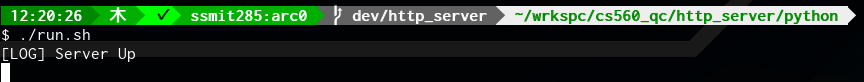
\includegraphics[width=\textwidth]{screenrun.png}
  \caption{The figure above shows the run command to start the web server and the result of the webserver running.}
\end{figure}
\FloatBarrier
\end{enumerate}

\section{Implementation Screenshots} 
\textbf{NOTE: We have already demoed to the TA for this course and have proven that our implementation of the HTTP web server is correct and in working order.}
     \begin{figure}[!htbp]
        \frame{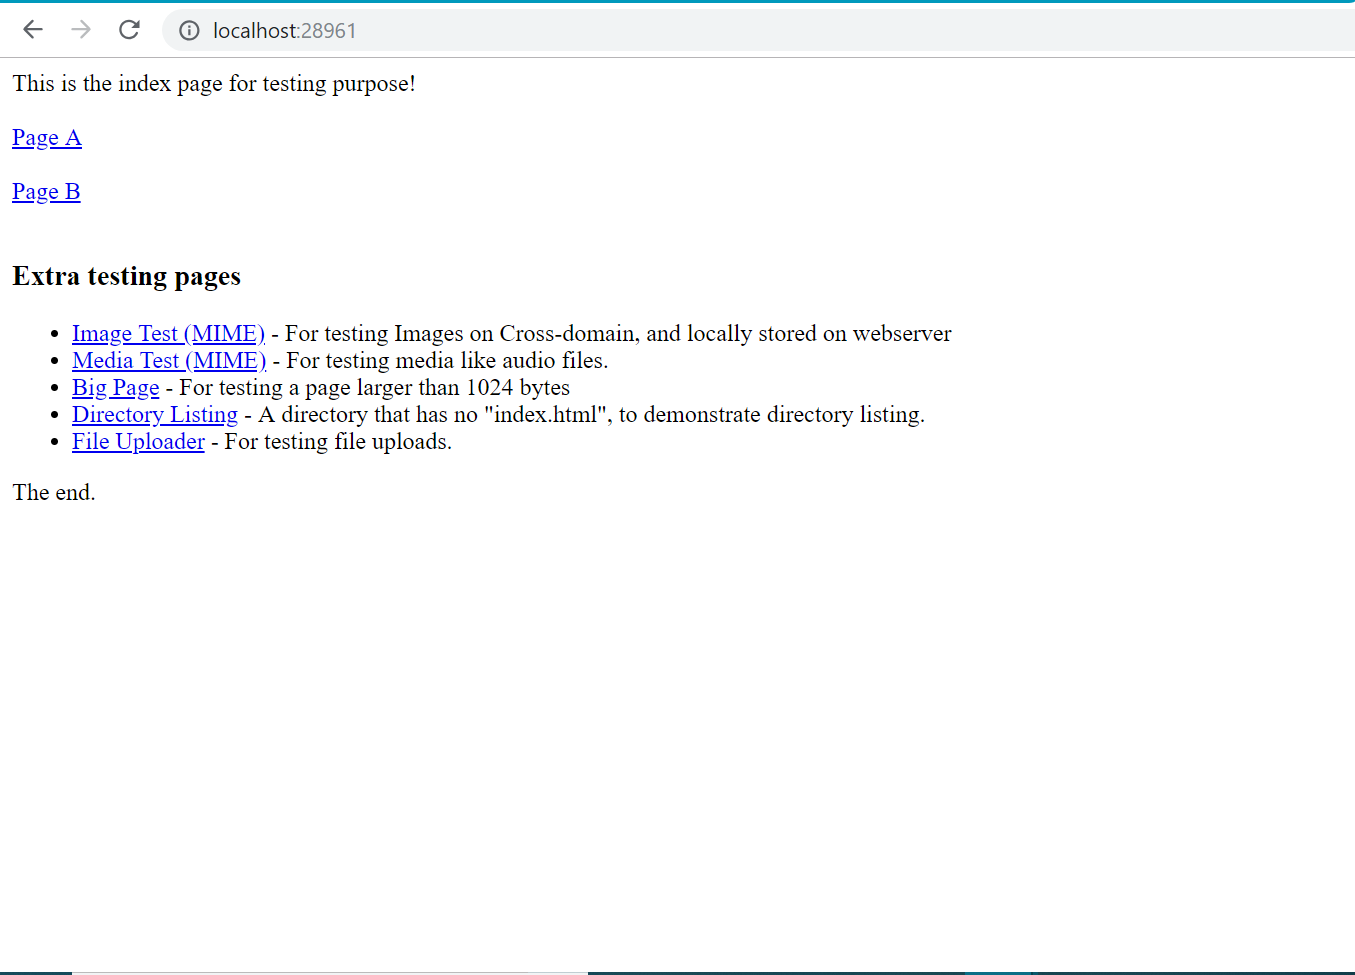
\includegraphics[width=\textwidth]{indexpage.PNG}}
        \caption{The figure above shows the index.html page of the webserver.}
    \end{figure}
         \begin{figure}[!htbp]
  \frame{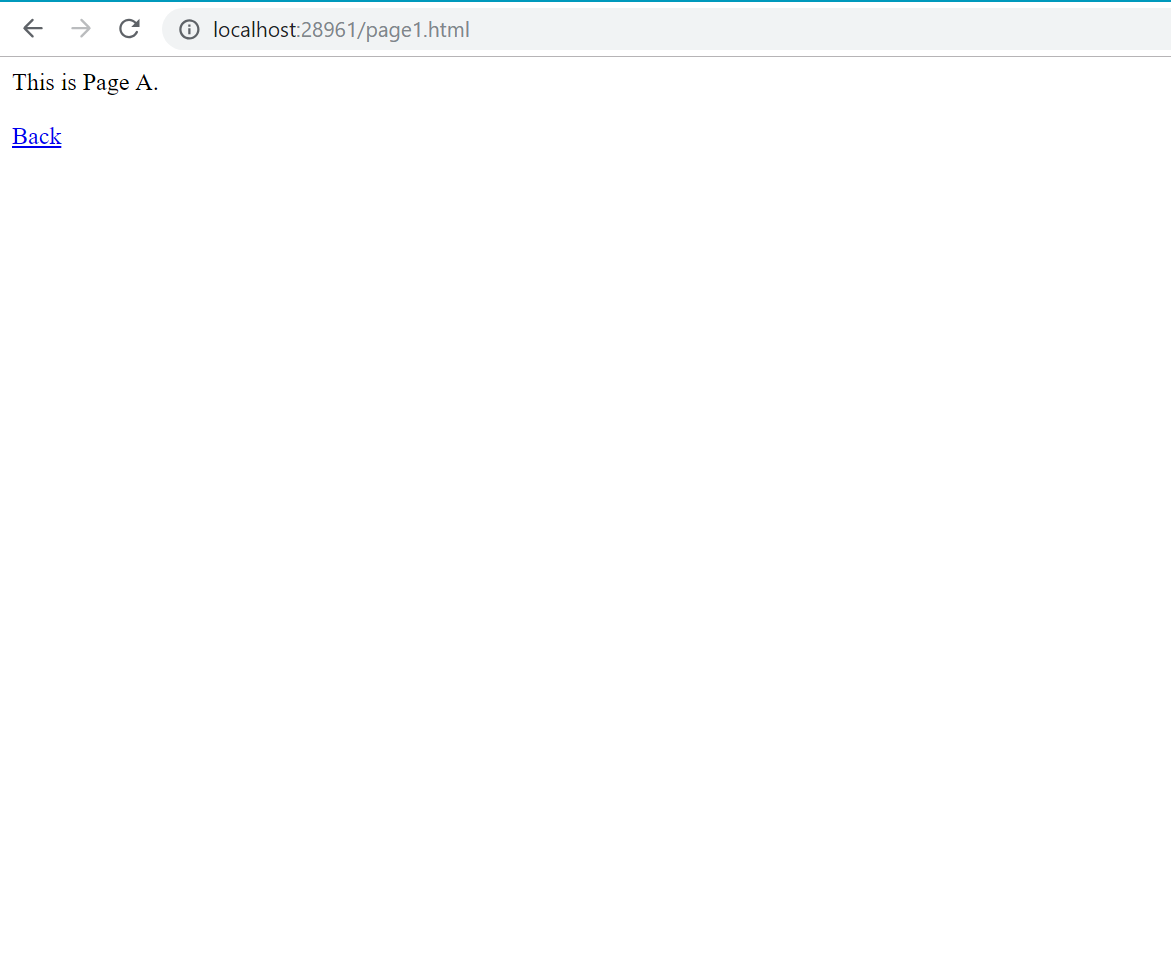
\includegraphics[width=\textwidth]{pageA.PNG}}
  \caption{The figure above shows the additional page, Page A, in the webserver.}
\end{figure}
     \begin{figure}[!htbp]
 \frame{ 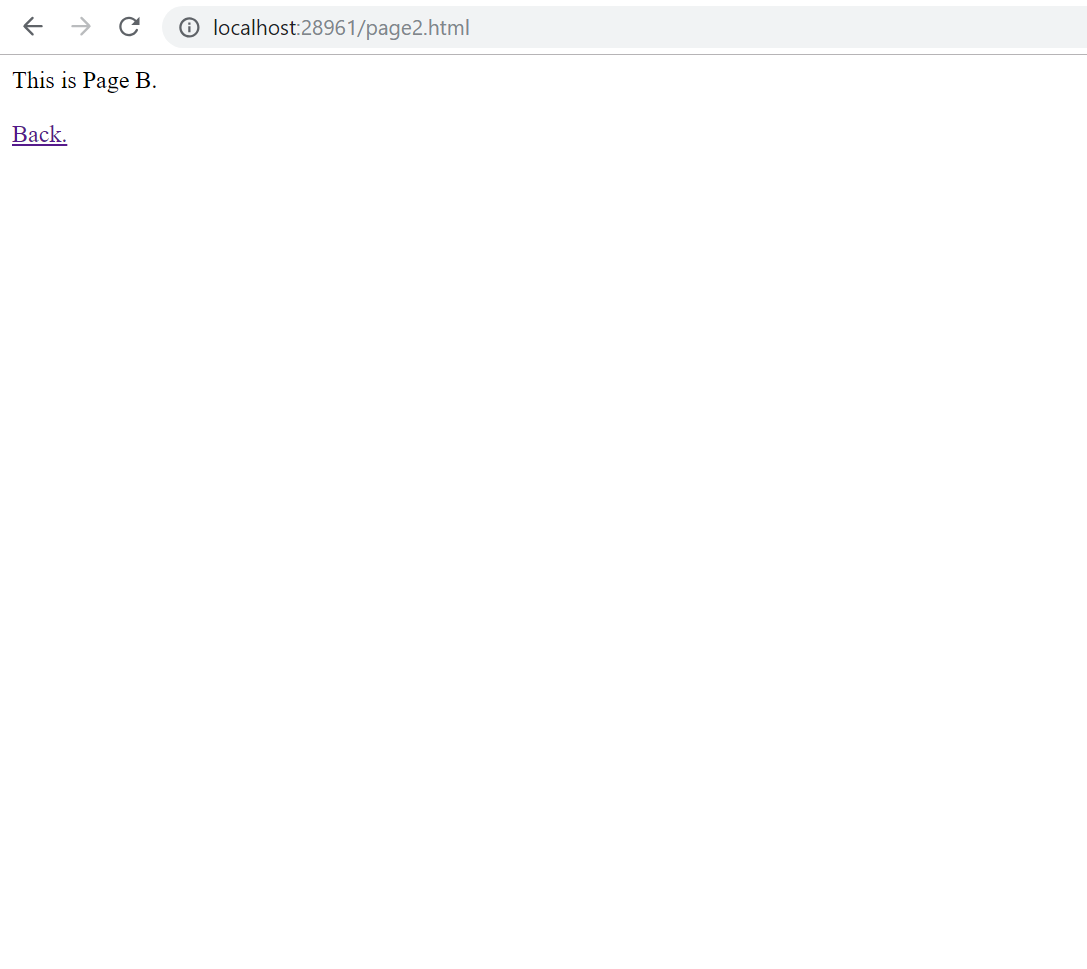
\includegraphics[width=\textwidth]{pageB.PNG}}
  \caption{The figure above shows the additional page, Page B, in the webserver.}
\end{figure}
     \begin{figure}[!htbp]
 \frame{ 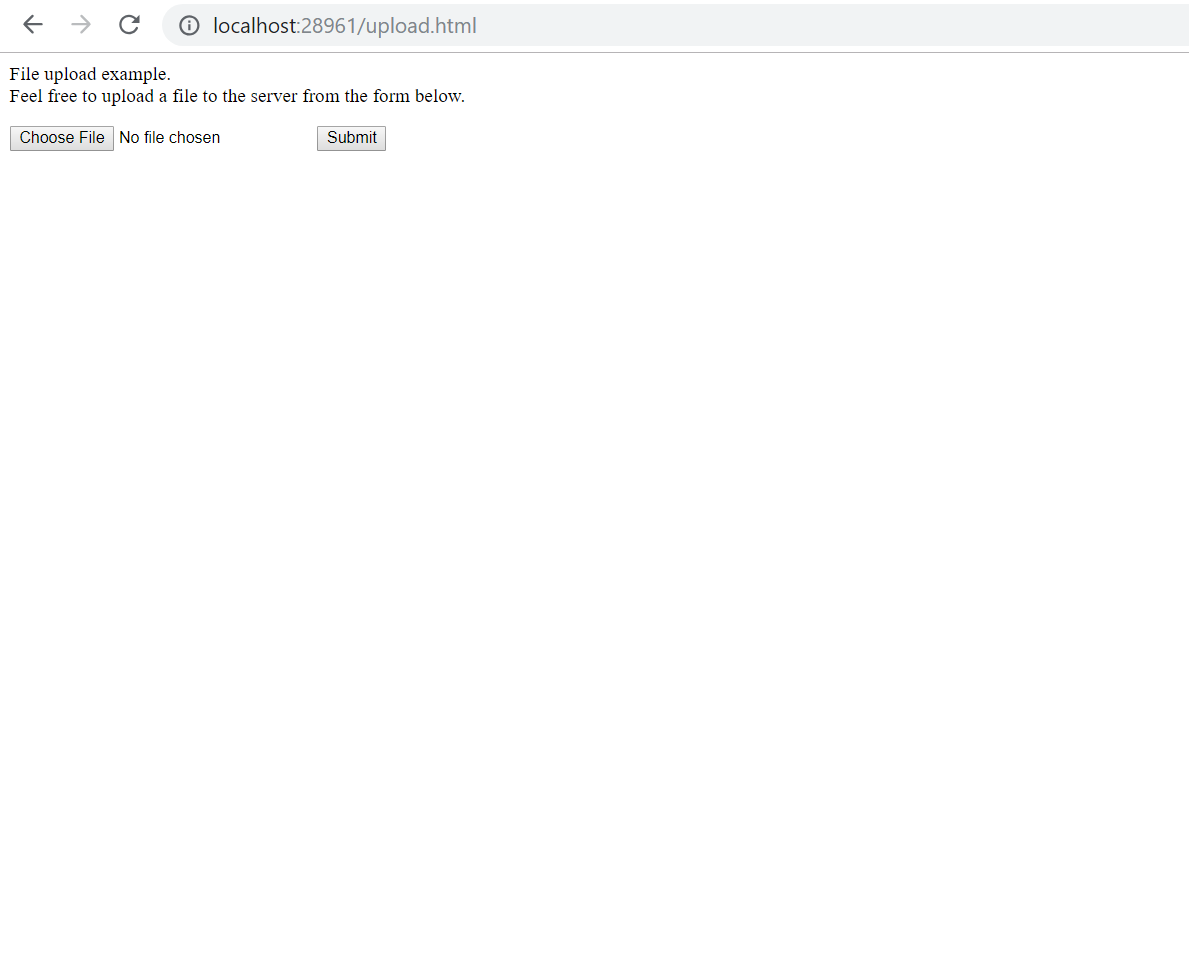
\includegraphics[width=\textwidth]{pageUpload.PNG}}
  \caption{The figure above shows the additional page, for uploading files.}
\end{figure}
     \begin{figure}[!htbp]
 \frame{ 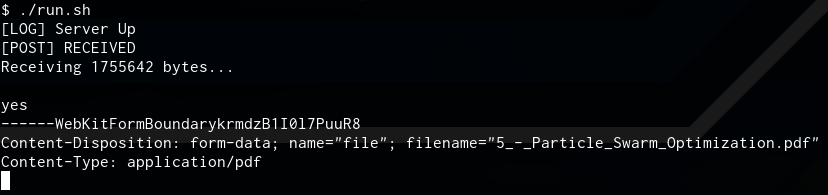
\includegraphics[width=\textwidth]{servergotfile.png}}
  \caption{The figure above that the server has received the request to upload the file.}
\end{figure}
     \begin{figure}[!htbp]
 \frame{ 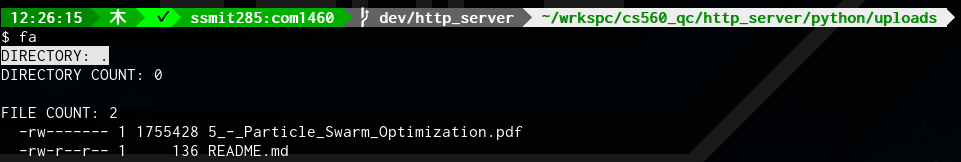
\includegraphics[width=\textwidth]{showserverhasfile.png}}
  \caption{The figure above shows that the server has uploaded the file and the file is now listed in the directory listing.}
\end{figure}
     \begin{figure}[!htbp]
 \frame{ 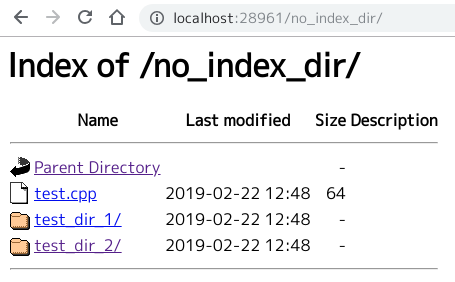
\includegraphics[width=\textwidth]{dirlist.png}}
  \caption{The figure above shows the directory listing page.}
\end{figure}
     \begin{figure}[!htbp]
 \frame{ 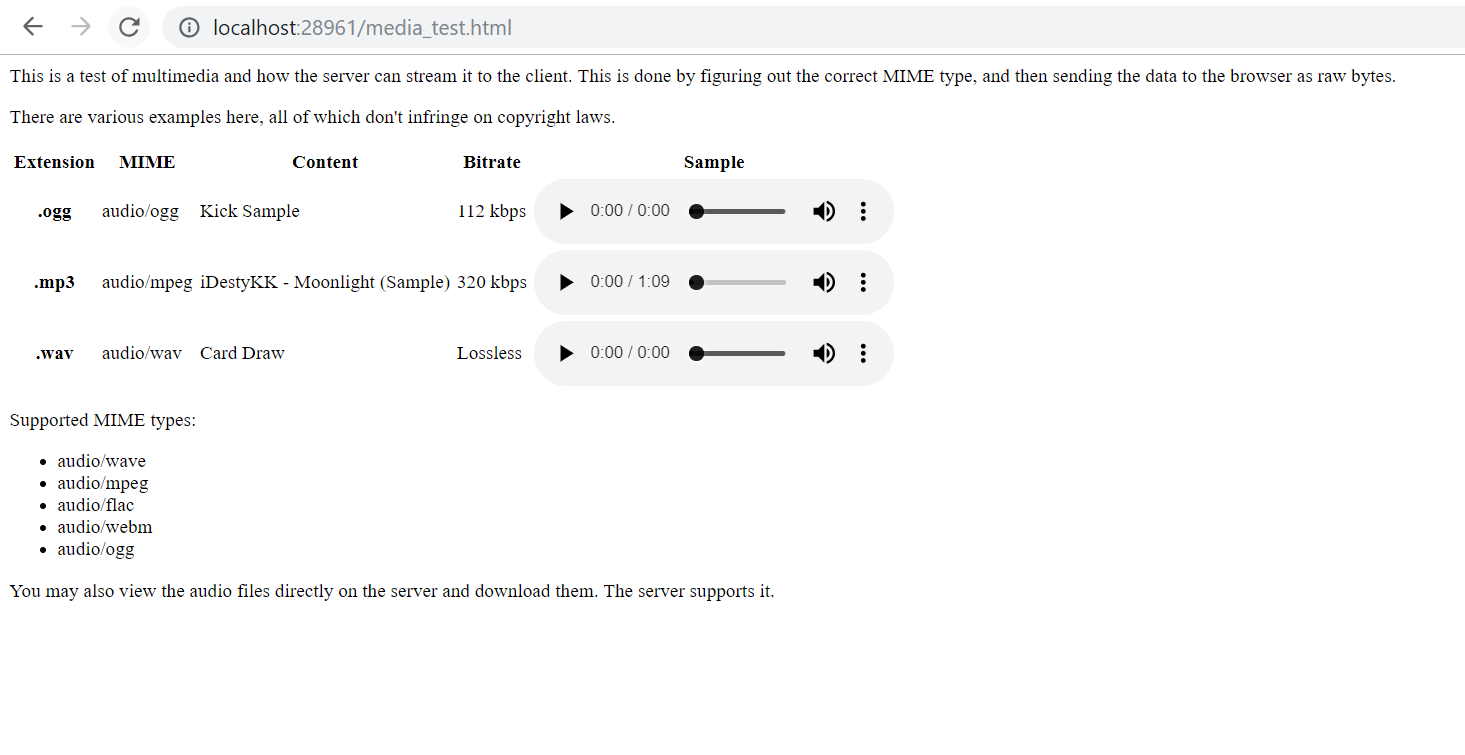
\includegraphics[width=\textwidth]{pageMedia.PNG}}
  \caption{The figure above shows the additional page, the Media Test Page, in the webserver. This was not a main requirement of the assignment, but was added in as an enhancement.}
\end{figure}
 \begin{figure}[!htbp]
 \frame{ 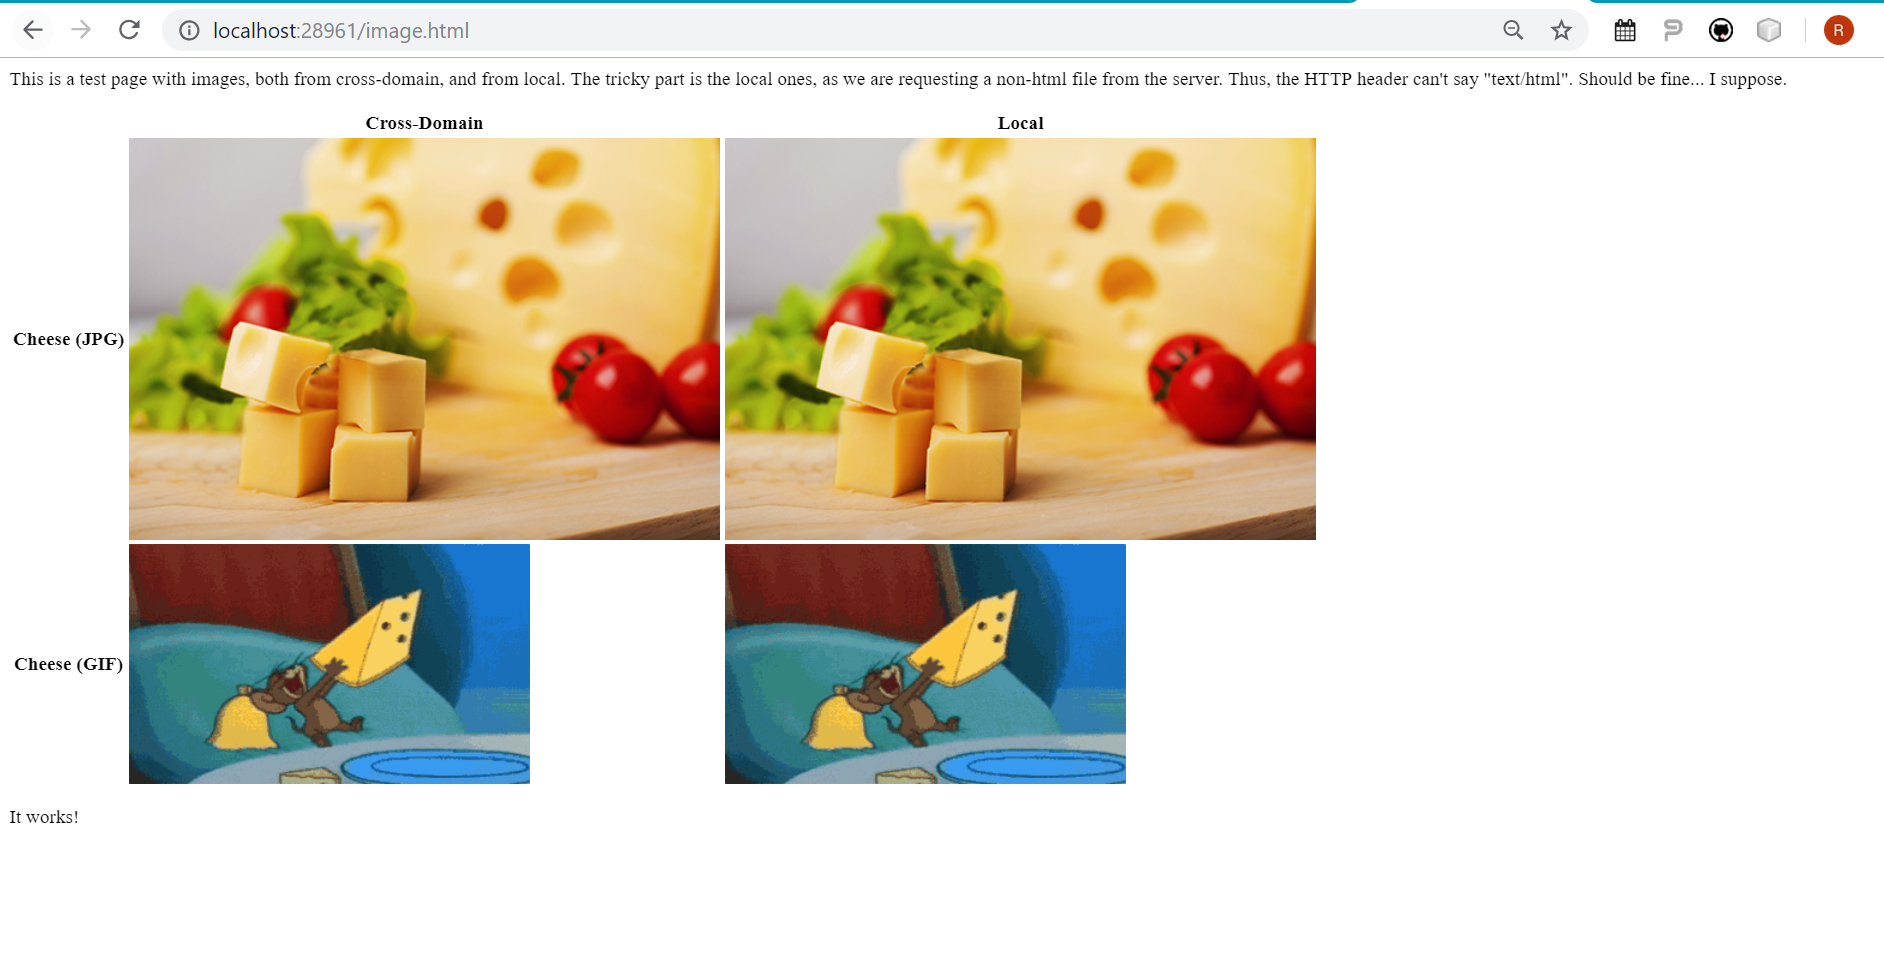
\includegraphics[width=\textwidth]{pageImage.PNG}}
  \caption{The figure above shows the additional page, the Image Test Page, in the webserver. This was not a main requirement of the assignment, but was added in as an enhancement. This page demonstrates locally hosted images and externally hosted images.}
\end{figure}



\end{document}

